\chapter{Related work} % Main chapter title
The research area of web crawling in general is big. In this thesis we want to focus on the work that has been done regarding architectures of web crawlers. Only a few have actually tried to build a scalable, parallel and distributed web crawler. The following sections present the different work that has been done organized by their idea.
\label{Chapter2} % Change X to a consecutive number; for referencing this chapter elsewhere, use \ref{ChapterX}
\lhead{Chapter 2. \emph{Related work}} % Change X to a consecutive number; this is for the header on each page - perhaps a shortened title

\section{Sequential crawlers}
One page is downloaded at the time. Nothing happens in parallel. Theses kind of web crawlers were used in the very beginning of the web. As the number of web pages grew the need to download web pages at a higher rate was obvious.

\section{Parallel centralized crawlers}
This kind of crawlers use several distinct components in their system. Each component is typically responsible for one or more specific tasks (ex. Downloader, Manager, Resolver). There is always one component that takes the role of a manager and is therefore \emph{central}. Such systems are more difficult to scale.

\subsection{Design and Implementation of a High-Performance Distributed Web Crawler~\cite{hp_crawler}}
This crawler design is separated into two main components, referred to as \emph{crawling application} and \emph{crawling system}. The crawling application decides which URLs to download next (ex. Breadth-first, focused), whereas the crawling system is responsible for handling the stream of URLs efficiently. Figure~\ref{hp_crawler} shows an overview of the system.
\begin{figure}[h]
\centering
  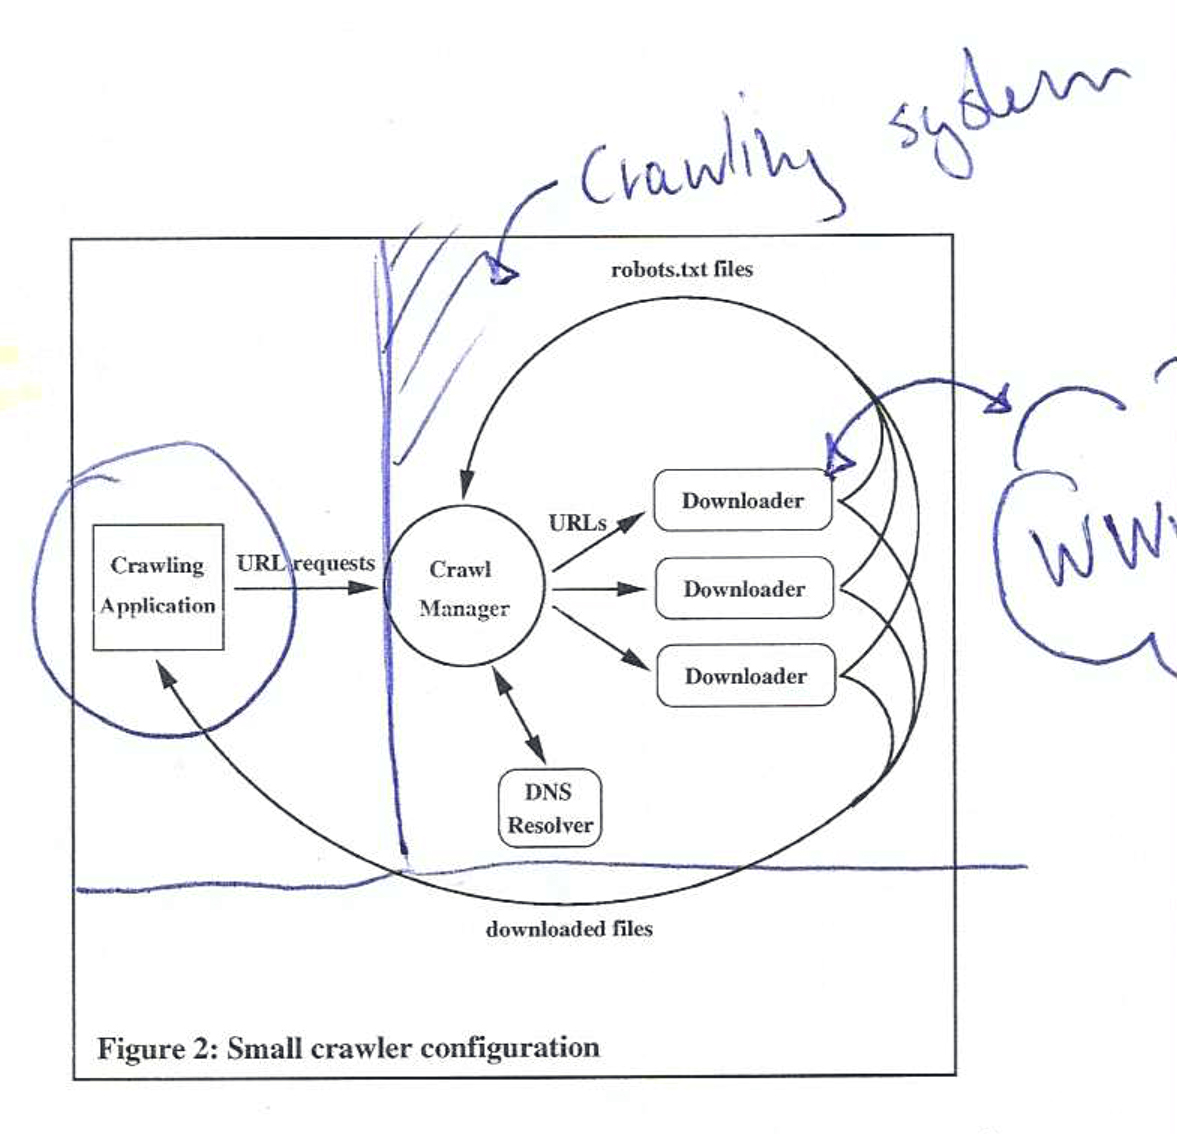
\includegraphics[width=0.7\textwidth]{Figures/hp_crawler.jpg}
\caption{System Architecture centralized crawler (High-Performance Distributed Web Crawler)}
\label{hp_crawler}
\end{figure}
As you can see `The crawl manager is the central component of the system'. Following the path of an URL (starting from the Crawl Manager) leads us to the \emph{Downloader} and back to the Crawling application. Scaling such a system is possible but requires more effort than in decentralized systems. How a larger system might look like is described in detail but we will not discuss it further because of other architectural design choices of Crawl.js.
Interestingly the details discussed in section \emph{Implementation Details and Algorithmic Techniques} revealed common problems and were of great use for Crawl.js. Parsing using regular expressions \footnote{\url{http://en.wikipedia.org/wiki/Regular_expression}} will be evaluated against regular parsing. And the sentence `We first note that fetching URLs in the order they were parsed out of the pages is a very bad idea, since there is a lot of second-level domain locality in the links' will be respected during the implementation phase. More details later. 

\section{Parallel decentralized crawlers}
Decentralized crawlers do not have a central managing unit. Typically those systems have identifiable and equal workers which are responsible for a certain piece of the work. Such a system is fully distributed and easily scalable (increase the number of workers). Of course there is some sort of communication between the workers (that could be seen as central), but the important point is that each worker is equal and autonomic.

\subsection{UbiCrawler: a scalable fully distributed Web crawler \cite{ubicrawler}}
UbiCrawler have multiple identically implemented (Java) workers (called agents). Every worker has an identity and is responsible for a defined set of URLs. For a given URL every worker is able to compute the identity responsible for that URL locally. This reduces the intercommunication overhead between the different workers in the system. The component used to compute a workers identity (based on a URL) is called \emph{assignment function}. It is important to note here, that the function directly assigns an identity of a worker. To be more precise, a worker that is alive and healthy. This fact of direct assignment leads to a problem UbiCrawler needs to solve. What happens if the assigned worker crashes? In this case it must be guaranteed that the function reassigns the same worker after he is back alive. (For a rapidly changing total set of URLs). So they need an assignment function that is:
\begin{itemize}
\item Random (to properly load balance the system)
\item Local (Problem of joining/leaving workers)
\item Contravariant (adding new workers, shrinks the workload (set of URLs) of one worker. )
\end{itemize}
Satisfying two of those requirements (Random, Contravariant) is easily achievable with a simple modulo function on the hash of the URL for example. The information every worker must know at anytime is the total number of workers in the system. Satisfying the third one is more complex and they solved it using a modified version of \emph{consistent hashing} called \emph{Identifier–Seeded Consistent Hashing}. 

Crawl.js will try to circumvent this complexity by adding an additional layer between the assignment function and the responsible worker. In Crawl.js the assignment function doesn't assign an identity of a worker but an identity of a bucket. A bucket is nothing more than a persistent queue. So the assignment function doesn't know anything about workers. In a second step Crawl.js will assign workers to those buckets. Using this additional layer removes complexity to the assignment function while keeping fault tolerance capabilities. This is achieved by flagging processed URLs within the bucket.
